\section{Moving} \label{moving}
A player's movement is defined by their Move score.
A player can only move up to their Move score, beyond that they have to do a \textit{sprint} action, which carries the risk of failure.

\subsection{Reach \& Blocking}
Every player has a zone around them, which makes up their \textit{reach} (see \figref{fig:tackle-zone-1}).
Their reach is made up of every hex immediately around them.

If an your player moves into or through the reach of an opposing player, they are said to be \textit{blocked}, and must perform a \textit{Dodge} check to keep moving (see \secref{skill-checks}).

\begin{note}
    Reaches can also overlap (see figure \ref{fig:tackle-zone-2}).
    If your player tries to move out of overlapping reaches, the opposing coach(es) may opt to have the players pile in (see \secref{dogpiling}).
\end{note}

\begin{figure}
    \centering
    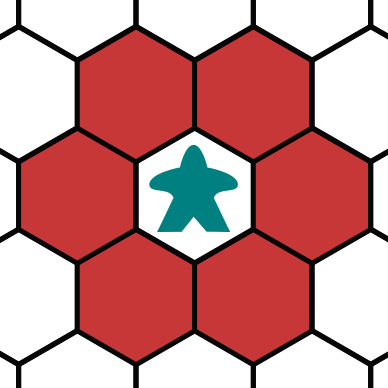
\includegraphics{graphics/tackle-zones-1.png}
    \caption{The reach around a player.}
    \label{fig:tackle-zone-1}
\end{figure}

\begin{figure}
    \centering
    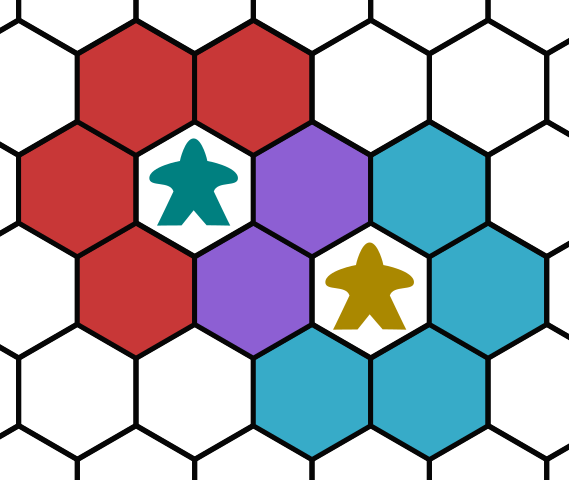
\includegraphics{graphics/tackle-zones-2.png}
    \caption{The overlapping reaches between two players.}
    \label{fig:tackle-zone-2}
\end{figure}